\documentclass[parskip=half]{scrartcl}

\usepackage[T1]{fontenc}
\usepackage[utf8]{inputenc}
\usepackage[english]{babel}

\usepackage[glows]{tikzpingus}
\usepackage[linkcolor=pingu@purple,urlcolor=pingu@purple,colorlinks,breaklinks,pdfusetitle]{hyperref}
\urlstyle{same}
\expandafter\def\expandafter\UrlBreaks\expandafter{\UrlBreaks\do-}

\usepackage[tex]{listings}
\usepackage[most]{tcolorbox}
\usepackage{imakeidx,tikz,fontawesome,csquotes,enumitem,microtype,tikzducks}
\newlist{inlist}{enumerate*}{1}
\setlist[inlist]{itemjoin={{,\space}},itemjoin*={{, and }},label=$\roman*$),mode=boxed}
\let\say\enquote
\usepackage{lmodern,CrimsonPro}

\addtokomafont{sectioning}{\color{gray}}
\addtokomafont{title}{\color{pingu@purple}}
\addtokomafont{author}{\normalsize}
\addtokomafont{date}{\normalsize}

\lstdefinestyle{lstpingu}{%
	tabsize=2, breaklines,
	basicstyle=\small\ttfamily,
	commentstyle={\color{gray}\slshape},
	columns=fullflexible,
	emphstyle=\slshape,
	alsoletter={ },
	emphstyle=[2]\color{pingu@blue!80!black}\slshape,
	texcsstyle=*\color{gray}\bfseries,
	texcsstyle=*[2]\color{pingu@purple}\bfseries,
	lineskip=2.5pt
}
\lstset{style=lstpingu}

\lstdefinelanguage{pingulang}{
	language={[LaTeX]TeX},
	moreemph={tikzpicture},
	alsoletter={-},
	moreemph=[2]{left,right,wing,eye,wings,eyes,shiny,wink,wave,grab,hug,wave,cup,xshift,yshift,meta,dots,name},
	moretexcs=[2]{pingu,duck,node},
	moredelim=[s][\itshape]{<}{>}
}

\tcbset{%
	colframe=gray,
	arc=2mm, arc is angular,
	fonttitle=\bfseries,
	sidebyside,
	listing options={style=lstpingu,language=pingulang},
	center lower,
	righthand width=5cm,
	bottom=0pt,top=0pt,
	before lower={\parskip.5cm},
}
\lstMakeShortInline[style=lstpingu,language=pingulang]{|}

\def\TikZ{Ti\textit{k}Z}
\def\tikzpingus{\TikZ pingus}

\title{The \texorpdfstring{\tikzpingus}{tikzpingus} package}
\subtitle{penguins in \TikZ}
\author{%
	\texorpdfstring{Florian Sihler\\[0.4em]
		\url{https://github.com/EagleoutIce/tikzpingus}
	}{Florian Sihler}}
\date{Version v1.0 \textendash\ 2021/07/02}

\begin{document}
\maketitle

\section{Motivation}
For my slides at university, I started to use the fairly famous \LaTeX-package \textsl{\href{https://github.com/samcarter/tikzducks}{tikzducks}}.
Yet, it seemed somewhat of a necessity to extend the range of available \say{cute} animals in \LaTeX.
Therefore I started writing this package: \textsl{tikzpingus}.\footnote{Why \say{pingu} and not \say{pengu}? Well, this is the third try on achieving cute penguins without using any templates or vector formats as a basis. As a german, the short form \say{pingu} was merely a typo that originated from the german word \say{pinguin} for \say{penguin}. It somewhat sticked\ldots}

\textit{Please note: } While tikzpingus is certainly inspired by tikzducks, it does offer a different set of features (e.g. multiple arm positions,~\ldots).

I would be happy for any feedback or issues on the \href{https://github.com/EagleoutIce/tikzpingus}{tikzpingus}-GitHub.

\subsection{Dependencies}

As this package is constantly work in progress, the concrete dependencies may change any time.
At the moment, it only loads \TikZ, which loads a lot of other packages (e.g. |xcolor|).
Furthermore, the following \TikZ-Libraries are in use:\footnote{A lot of the libraries loaded are important only for specific extras. I plan on cleaning them up.}
\begin{inlist}
	\item |intersections|
	\item |shadings|
	\item |patterns.meta|
	\item |decorations.pathmorphing|
	\item |shapes.symbols|
\end{inlist}.

\subsection{Copyright}

Copyright \textcopyright \texttt{Florian Sihler}. Permission is granted to copy, distribute and\slash or modify this software under the terms of the LaTeX project public licence, version 1.3c or later \url{http://www.latex-project.org/lppl.txt}.

The shown example penguins are purely fictional characters, any resemblance to real penguins or persons is purely coincidental and no copyright infringement is intended.

\section{Usage}

If you just want a penguin, use the following syntax:
\begin{tcblisting}{title={One small penguin}}
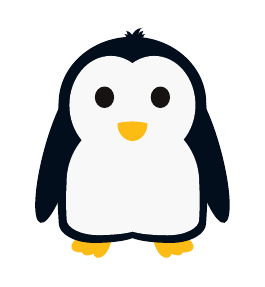
\begin{tikzpicture}
	\pingu
\end{tikzpicture}
\end{tcblisting}

There are \textit{a lot} of configuration-options which can be passed as an optional argument via the known |<key>=<value>|-style.
% TODO: click reference to full list; TODO: glow option
\begin{tcblisting}{title={Happy penguin with cup!}}
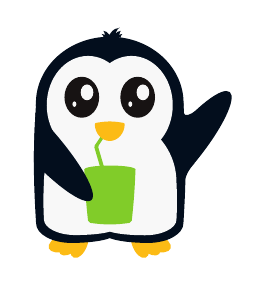
\begin{tikzpicture}
	\pingu[left wing wave, right wing grab,
	       eyes shiny, cup]
\end{tikzpicture}
\end{tcblisting}
Please note, that \say{left} and \say{right} have been chosen from the penguin-perspective.

Besides the keys defined by this package, you can use the keys of \TikZ\ and |pgf| as well (the duck was generated by the lovely \href{https://github.com/samcarter/tikzducks}{tikzducks} package):
\begin{tcblisting}{title={The Reunion}}
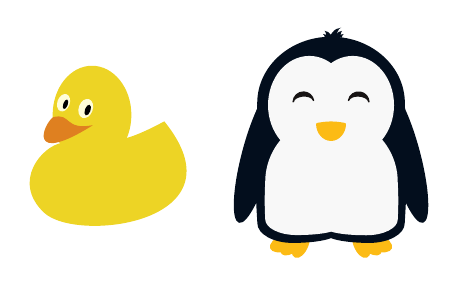
\begin{tikzpicture}
	\duck
	\pingu[xshift=3cm, yshift=14mm,
	       eyes wink]
\end{tikzpicture}
\end{tcblisting}
\subsection{Coordinates}
While there are a lot of gadgets available already,
every penguin is accompanied by \textit{a lot} of adaptive coordinates
to place custom items, texts,~\ldots\ % TODO: links
They can be placed by the meta-dots option and change their positions, angles,~\ldots\ depending on other options.
Furthermore, some extras create further coordinates themselves!
All coordinates are available with |<pigu-name>-<coordinate>|.
While the default name of a penguin is \say{pingu}, it can be
changed with the name option:
\begin{tcblisting}{title={Lotta dots}}
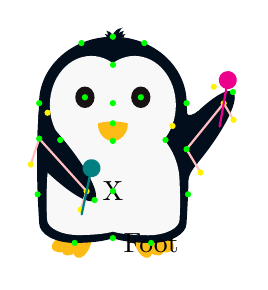
\begin{tikzpicture}
	\pingu[meta dots,left wing wave,
	       right wing grab, name=paula]
	\node at (paula-belly-center) {X};
	\node at (paula-foot-left) {Foot};
\end{tikzpicture}
\end{tcblisting}
Lets look at those coordinates in more detail (all labels are to be prefixed by |<pingu-name>-|):
\newsavebox\pinguwingright
\savebox\pinguwingright{%
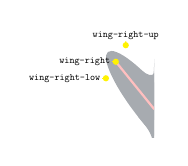
\begin{tikzpicture}%
	\scope
	\path[clip] (0,-.7) rectangle (-1,.7);
	\pgfonlayer{foreground}\path[clip] (0,-.7) rectangle (-1,.7);\endpgfonlayer
	\pingu[@block/.append style={fill=#1!35!white}, wings wave,eyes shiny,heart=gray!30!white,feet=none]
	\path[draw,pink,thick] (pingu-wing-right-start) -- (pingu-wing-right);
	\endscope
	\foreach \c/\a in {wing-right/left,wing-right-low/left,wing-right-up/above} {
		\path[fill=yellow] (pingu-\c) circle [radius=1.125pt];
		\node[\a=.5mm,font=\ttfamily,scale=.35,inner sep=1.5pt] (expl-\c) at (pingu-\c) {\c};
		\draw[yellow,thin] (expl-\c) -- (pingu-\c);
	}
\end{tikzpicture}%
}
\makeatletter
\newsavebox\pinguwingleft
\savebox\pinguwingleft{%
\begin{tikzpicture}%
	\scope
	\path[clip] (\pingu@w@half*2,-.7) rectangle ++(1,1.4);
	\pgfonlayer{foreground}\path[clip] (\pingu@w@half*2,-.7) rectangle ++(1,1.4);\endpgfonlayer
	\pingu[@block/.append style={fill=#1!35!white}, wings wave,eyes shiny,heart=gray!30!white,feet=none]
	\path[draw,pink,thick] (pingu-wing-left-start) -- (pingu-wing-left);
	\endscope
	\foreach \c/\a in {wing-left/left,wing-left-low/below,wing-left-up/above} {
		\path[fill=yellow] (pingu-\c) circle [radius=1.125pt];
		\node[\a=.5mm,font=\ttfamily,scale=.35,inner sep=1.5pt] (expl-\c) at (pingu-\c) {\c};
		\draw[yellow,thin] (expl-\c) -- (pingu-\c);
	}
\end{tikzpicture}%
}

\begin{center}
	\resizebox{.9\linewidth}!{
		\begin{tikzpicture}
			\pingu[@block/.append style={fill=#1!35!white}, wings wave,eyes shiny,heart=gray!30!white]
			\pgfonlayer{foreground}
			\foreach \c/\a in {belly-center/above,head/below,head-top/above,foot-left/right,foot-right/left,right-eye/above left,left-eye/above right,bill/right,bill-bottom/below,wings-side-left/right,wings-side-right/left,wing-left-start/below right,wing-left-tip/right,wing-right-start/below left,wing-right-tip/left,head-right/left,head-left/right,head-center/below,head-back-con-left/right,head-back-con-right/left,bottom-center/above,waist-left/right,waist-right/left} {
				\path[fill=green] (pingu-\c) circle [radius=1.125pt];
				\node[\a=.5mm,font=\ttfamily,scale=.35,inner sep=1.5pt] (expl-\c) at (pingu-\c) {\c};
				\draw[green,thin] (expl-\c) -- (pingu-\c);
			}
			\endpgfonlayer
		\end{tikzpicture}
	}
\end{center}
\paragraph{The Wings}
This view excluded a lot of special data collected on the wings!
While there is more information stored for each wing, the following three coordinates are the most important to place items into penguins hand:
\begin{center}
	\null\hfill\scalebox2{\usebox\pinguwingright}\hfill
	\scalebox2{\usebox\pinguwingleft}\hfill\null
\end{center}

\end{document}